\chapter{Experimental Results}\label{sec:results}

\begin{quote}
    In this chapter, we outline the results obtained from the experiments and detail the outcomes of the ablation study. The quality of our models' representations are evaluated with the music classification task.
\end{quote}

\begin{table}
    \centering
    \begin{tabular}{@{}llcc@{}}\toprule
        Model & Dataset & $\text{ROC-AUC}_\text{TAG}$ & $\text{PR-AUC}_\text{TAG}$ \\ \midrule
        % \multicolumn{4}{c}{MTAT-Trained Experiments}\\\addlinespace
        CLMR (ours) & MTAT & 88.49 (\textbf{89.25}) & \textbf{35.37} (\textbf{35.89}) \\
        Pons et al.$^\dagger$ & MTAT & 89.05 & 34.92 \\
        SampleCNN$^\dagger$ & MTAT & 88.56 & 34.38 \\
        CPC (ours) & MTAT & 86.60 (87.99) & 30.98 (33.04) \\
        1D CNN$^\dagger$ & MTAT & 85.58 & 29.59 \\\midrule
        Pons et al.$^\dagger$ & MSD & 87.41 & \textbf{28.53} \\
        SampleCNN$^\dagger$ & MSD & \textbf{88.42} & - \\
        CLMR (ours) & MSD & 85.66 & 24.98 \\
        \bottomrule
    \end{tabular}
    \caption{Tag prediction performance on the MagnaTagATune (MTAT) dataset and Million Song Dataset (MSD), compared with fully supervised models$^\dagger$ trained on raw audio waveforms.
    We omit works that operate on audio in the time-frequency domain.
For the supervised models, the tag-wise scores are obtained by end-to-end training.
For the self-supervised models, the scores are obtained by training a \emph{linear}, logistic regression classifier using the representations from self-supervised pre-training.
Scores in parenthesis show performance when adding one hidden layer to the logistic regression classifier, making it a simple multi-layer perceptron.}
    \label{tab:results}
\end{table}


\section{Quantitative Evaluation}
The most important goal set out in this thesis, was to evaluate the difference in performance between a fully supervised and fully unsupervised objective when learning representations, using the exact same encoder set-up. The CLMR model in our experiments uses the SampleCNN encoder network. When SampleCNN is trained in a fully supervised manner, it reaches an PR-AUC score of 34.92. CLMR exceeds this supervised benchmark with a PR-AUC of 35.37, despite task-agnostic, self-supervised pre-training and a \textit{linear} classifier for fine-tuning. An additional 0.5\% performance is added by adding one extra hidden layer to the classifier. Evaluation scores of the best-performing CLMR, CPC and other wave-form based models are shown in Table \ref{tab:results}.

CLMR also outperformed the current state-of-the-art waveform-based model in the task of automatic music tagging \cite{pons_end--end_2017} in both evaluation metrics for the MagnaTagATune dataset.

The performance on the Million Song Dataset is lower than that of SampleCNN. The highest evaluation scores for the MagnaTagATune dataset were obtained after very long pre-training ($\leq 10000$ epochs). While this was feasible for a dataset of the size of MagnaTagATune's, We did not have the equipment available to run the experiment for so long on the Million Song Dataset.

CPC also shows competitive performance with fully supervised models in the music classification task, despite being pre-trained without ground truth and using a simple, linear classifier for evaluation.
Despite CPC's good performance, self-supervised training indeed does not require a memory bank or more complex loss functions, e.g., those incorporating mutual information or more explicit negative sampling strategies, to learn useful representations.


\section{Qualitative Analysis}
For a qualitative view of the representations, we show how cleanly they are  separable using a $t$-SNE manifold in Figure \ref{fig:tsne_manifold}.
Figure \ref{fig:tag_scores} shows in more detail that the difference in performance between self-supervised and supervised models is marginal: there is no single tag performance difference larger than 4\% ROC-AUC, and for practical purposes, CLMR and CPC retrieve tags practically identically to supervised models.

\begin{figure}[h]
    \centering
    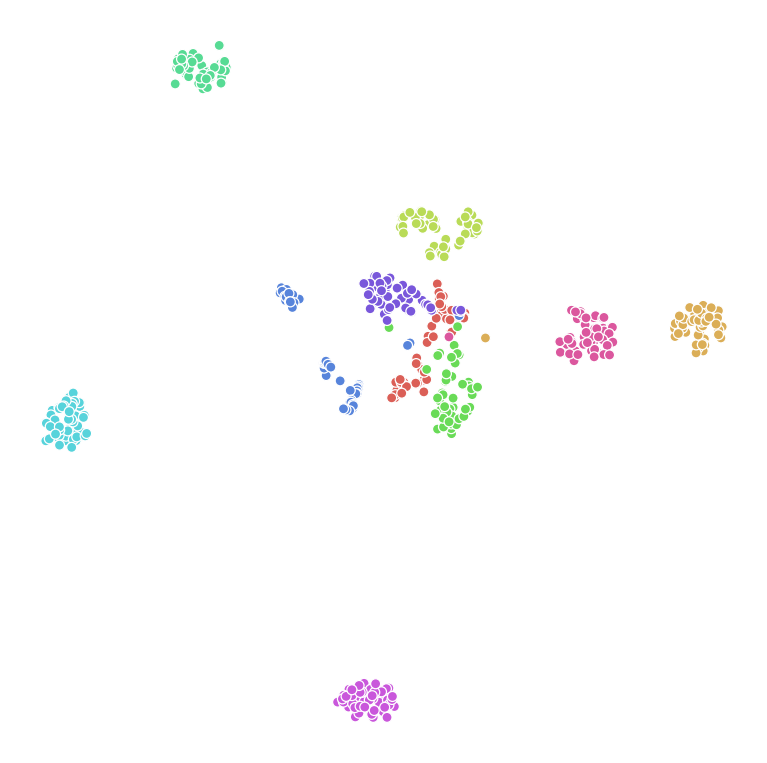
\includegraphics[width=0.75\textwidth]{figs/tsne-clmr.png}
    \caption{$t$-SNE manifold visualisation from audio representations learned by a converged CLMR model of a subset of 10 tracks with each 60 segments.
Every color represents a separate track.}
    \label{fig:tsne_manifold}
\end{figure}

\begin{figure*}[h]
    \centering
    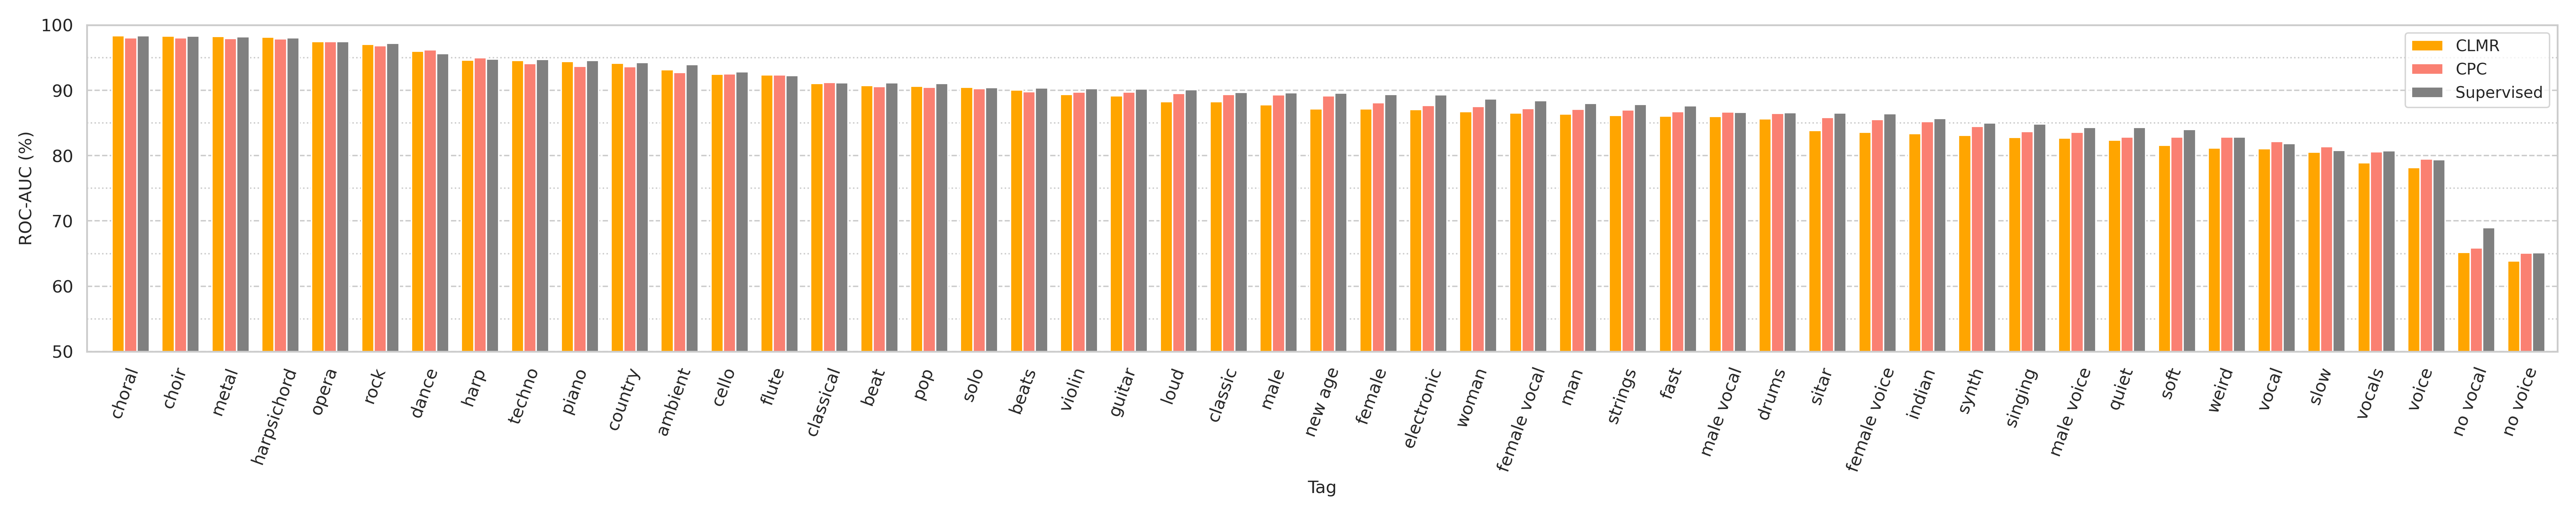
\includegraphics[width=\textwidth]{figs/tag_retrieval.png}
    \caption{Tag-wise ROC-AUC scores for the top-50 tags in the MagnaTagATune dataset, reported for linear, logistic regression classifiers trained on representations of self-supervised models CLMR and CPC, and compared to a fully supervised, end-to-end SampleCNN model.}
    \label{fig:tag_scores}
\end{figure*}


\section{Data Augmentations}
The CLMR model relies on a pipeline of strong data augmentations to facilitate the learning of representations that are more robust and allow for better generalisation in the downstream task.
In Figure \ref{fig:transformation_study}, we show the PR-AUC linear evaluation score that is achieved when taking a random slice of audio (`random cropping') and performing one additional, individual augmentation.
While all datasets contain songs of variable length, we always sample a random slice of audio of the same size before applying other augmentations.
Since we always have to take a random slice, it makes it harder to assess the individual contribution of each augmentation to the downstream task performance.
We therefore consider an asymmetric data transformation setting: we only apply the augmentation pipeline to one branch of the framework, while we settle with an identity function for the other branch (i.e., $t(x_j) = x_j$) \cite{chen_simple_2020}. The transformations on the augmentation branch are applied with probability $p_t=1$, i.e., the transformation is always applied.

When only taking a random slice of audio (i.e., a `crop'), we achieve a PR-AUC score of $30.5$.
Most augmentations show a similar increase in performance of $±31.5$, while adding gain or delay does not impact performance as much.
Adding a filter to the pipeline increases the downstream performance significantly.

\begin{figure*}[h]
    \centering
    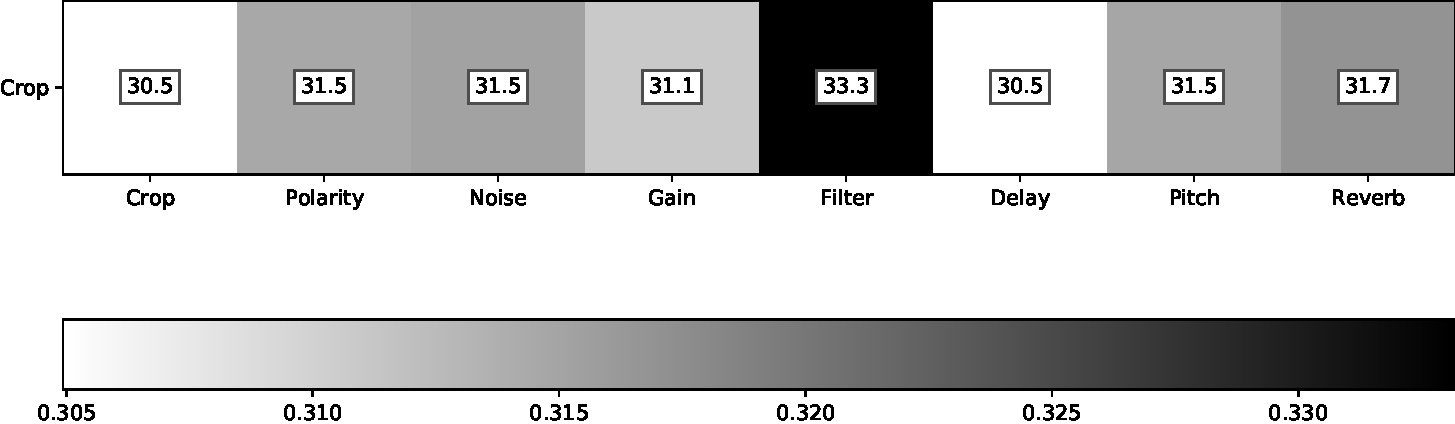
\includegraphics[width=\columnwidth]{figs/transformation_study.pdf}
    \caption{The achieved $\mathrm{PR-AUC}_{\mathrm{TAG}}$ score using a random crop transformation together with another TODO}
    \label{fig:transformation_study}
\end{figure*}

Besides evaluating the individual contribution of each augmentation with a probability of $p_t = 1$, we also vary this probability: $p_t \in \{ 0, 0.4, 0.8 \}$.
This is done to assess the optimal amount of augmentation to each example, i.e., the contrastive learning task should not be too hard, neither too simple, for learning effective representations in the downstream music classification task.
The linear evaluation PR-AUC score is shown for each augmentation under a different probability $p_t$ in Figure \ref{fig:transformation_probabilities}. For the Polarity and Filter transformations, performing them more often with a probability of $p_t = 0.8$ is beneficial. For the Delay, Pitch and Reverb transformations, a transformation probability of $p_t = 0.4$ works better than performing them more aggressively.

\begin{figure}[h]
    \centering
    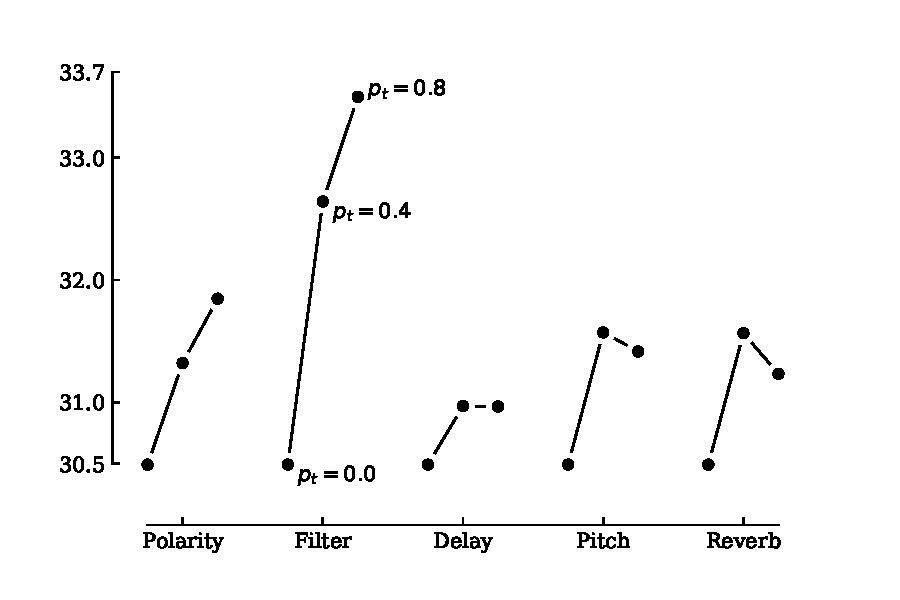
\includegraphics[width=\columnwidth]{figs/transformation_probabilities.pdf}
    \caption[-5cm]{$\mathrm{PR-AUC}_{\mathrm{TAG}}$ scores for transformations under different, consecutive probabilities $p \in \{ 0.0, 0.4, 0.8 \}$}
    \label{fig:transformation_probabilities}
\end{figure}


\section{Mini-Batch Size}
Increasing the batch size to 192 and 128 respectively also increases final evaluation scores.
We refer the reader to the supplementary material for a complete overview of the results obtained with different augmentation and model parameters.



\section{Additional experiments}
\subsection{Sample Rates}    
When re-sampling the audio to 8\,000~Hz and 16\,000~Hz respectively, there is a marginal penalty to the final scores for the self-supervised models, which is in line with previous work\cite{lee2018samplecnn}. In Table \ref{tab:sample_rate_ablation}, we show all linear evaluation scores when no additional transformations are performed (i.e., only random cropping) to isolate the contribution of each individual sample rate.


\begin{table*}
    \centering
        \begin{tabular}{lllll}\toprule
        Sample rate & $\text{ROC-AUC}_{\text{TAG}}$ & $\text{PR-AUC}_{\text{TAG}}$ & $\text{ROC-AUC}_{\text{CLIP}}$ & $\text{PR-AUC}_{\text{CLIP}}$ \\\midrule
        8000 & 84.78 & 29.77 & 90.60 & 62.94 \\
        16000 & 85.46 & 30.42 & 90.97 & 64.08 \\
        22050 & 85.82 & 30.49 & 91.25 & 64.78 \\                       
        \bottomrule
        \end{tabular}
    \caption[][24pt]{Effect of the sample rate on tag prediction performance.}
    \label{tab:sample_rate_ablation}
\end{table*}


% \subsection{Projector Network}
% A non-linear projector network positively impacts the performance of the model.
% Adding only one extra hidden layer to the classifier increases the results by $4\%$, making the gap between supervised end-to-end baselines even smaller.
% It is clear from these results that useful representations can be learned from high-dimensional signals of raw audio even without access to ground truth labels.

\subsection{Temperature}
The temperature parameter $\tau$ in the NT-Xent loss function (Equation \ref{eq:loss_function}) controls the penalty given to the negative samples. The experiments in Table \ref{tab:temperature_ablation} were run using a mini-batch size of 96, which is a smaller mini-batch size than those used in the original SimCLR paper (i.e., $\leq 4096$ samples per mini-batch) \cite{chen_simple_2020}. Consequently, the performance difference is marginal. Again, no additional transformations except random cropping were applied in this experiment to isolate the contribution of this temperature parameter.

\begin{table*}
    \centering
    \begin{tabular}{lllll}\toprule
    Temperature & $\text{ROC-AUC}_{\text{TAG}}$ & $\text{PR-AUC}_{\text{TAG}}$ & $\text{ROC-AUC}_{\text{CLIP}}$ & $\text{PR-AUC}_{\text{CLIP}}$ \\\midrule
    0.1         & 85.82                         & 30.33                        & 91.18                          & 64.10                         \\
    0.3         & 85.58                         & 30.35                        &                                &                               \\
    0.5         & 85.82                         & 30.49                        & 91.25                          & 64.78 \\                       
    \bottomrule
    \end{tabular}
    \caption[][24pt]{Ablation study of the temperature parameter in the NT-Xent loss function.}
    \label{tab:temperature_ablation}
\end{table*}


\section{Efficient Classification Experiments}
Figure \ref{fig:perc_train_data_magnatagatune} and \ref{fig:perc_train_data_msd} show the PR-AUC scores obtained when increasing the amount of labels available during fine-tuning.
For both datasets, fine-tuning using just $1\%$ of the labels yields a large performance difference compared to training in a fully supervised manner (using the same amount of labels).
Pre-training using a self-supervised objective without labels therefore substantially improves efficient classification: only $1\%$ of the labels are required while maintaining a similar performance.

For the Million Song Dataset, a fully supervised end-to-end model exceeds CLMR at $10\%$ of the labels, but we would like to note that our best CLMR model trained on the Million Song Dataset did not converge due to time- and hardware constraints.

\begin{figure}[h]
    \centering
    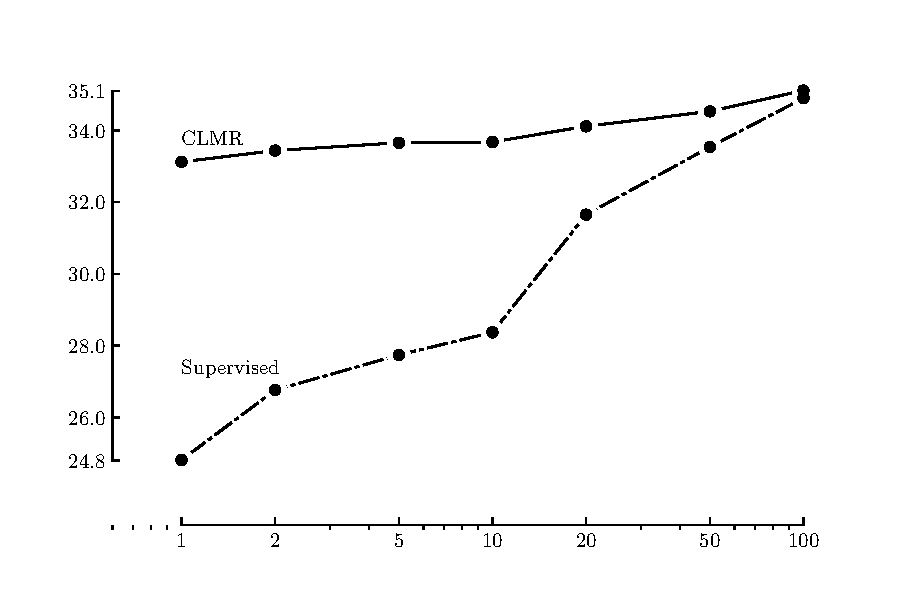
\includegraphics[width=\columnwidth]{figs/perc_train_data_magnatagatune.pdf}
    \caption{Percentage of labels used for training vs. the achieved $\mathrm{PR-AUC}_{\mathrm{TAG}}$ score on the MagnaTagATune dataset}
    \label{fig:perc_train_data_magnatagatune}
\end{figure}

\begin{figure}[h]
    \centering
    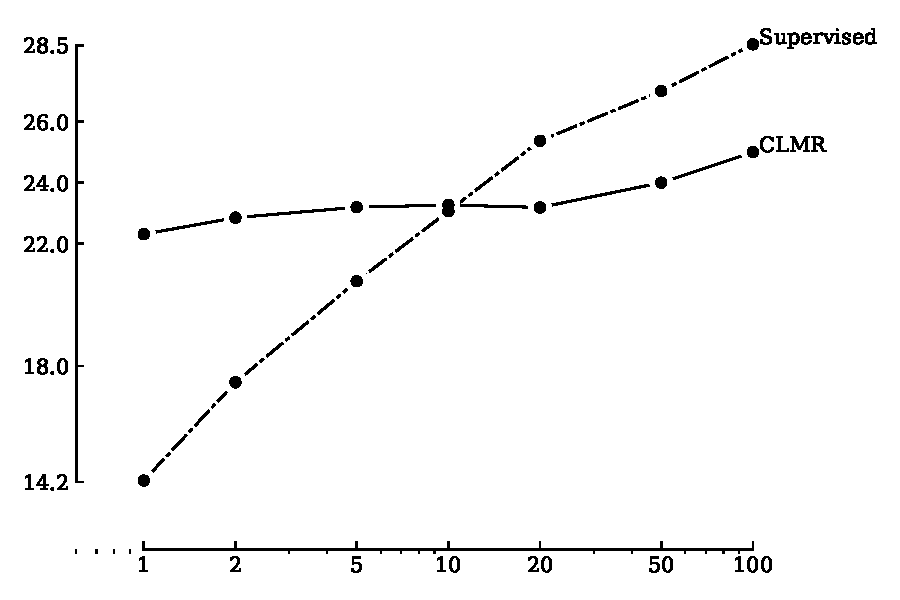
\includegraphics[width=\columnwidth]{figs/perc_train_data_msd.pdf}
    \caption{Percentage of labels used for training vs. the achieved $\mathrm{PR-AUC}_{\mathrm{TAG}}$ score on the Million Song Dataset.}
    \label{fig:perc_train_data_msd}
\end{figure}



\section{Transfer Learning Experiments}
The results of the transfer learning experiments are shown in Table \ref{tab:magnatagatune_results}.
Both CPC and CLMR show the ability to learn effective representations from datasets different from the evaluation dataset without ground truth, and even exceed accuracy scores of previous, supervised end-to-end systems on raw audio \cite{dieleman2014end}.
Moreover, both models demonstrate the ability to learn useful representations on small datasets like GTZAN.
The CLMR model performs better when pre-trained on larger datasets, which is expected as it heavily relies on the number of unique, independent examples to create correlated augmentations.
When pre-training on smaller datasets, the autoregressive modelling in CPC can find more useful representations for downstream tasks.
%contribute to more useful representations for downstream tasks.

\begin{table}[h]
    \centering
    \begin{tabular}{@{}lllcc@{}}\toprule
        Model & Train Dataset & Eval.
        Dataset &  ROC-AUC & PR-AUC \\ \midrule
        CLMR & MSD & MTAT &  \textbf{86.57} & \textbf{32.04} \\
        CPC & FMA & MTAT & 86.34 (\underline{87.79}) & 30.71 (\underline{32.47}) \\
        CLMR & FMA & MTAT & 86.22 (86.63) & 30.58 (31.22) \\
        CPC & Billboard & MTAT & 85.78 (86.25) & 29.68 (30.15) \\
        CPC & GTZAN & MTAT & 83.44 (86.06) & 26.88 (29.72) \\
        CLMR & Billboard & MTAT & 82.73 (84.22) & 26.86 (27.82) \\
        CLMR & GTZAN & MTAT & 81.88 (85.43) & 26.18 (29.49) \\
        \bottomrule
    \end{tabular}
    \caption{Performance of the self-supervised models when pre-trained on datasets different from the evaluation dataset, again using a linear classifier to evaluate.}
    \label{tab:magnatagatune_results}
\end{table}


